\documentclass[../../../../main.tex]{subfiles}

\begin{document}

\section*{第1問}

\noindent
[\textbf{解}]
\begin{align}
x^3 - y^3 - z^3 &= 3xyz \tag{1} \\
x^2 &= 2(y + z) \tag{2}
\end{align}
(2)を(1)に代入して
\begin{align}
\{ 2(y+z) - 3yz \} x = y^3 + z^3 \tag{3}
\end{align}
$x, y, z \in \mathbb{N}$ から $x > 0, y^3 + z^3 > 0$ だから $2(y+z) - 3yz > 0$ が必要。対称性から $y \le z$ とすると
\[
3yz < 2(y+z) \le 4z \quad \therefore 3y < 4 \quad (\because z > 0)
\]
$y \in \mathbb{N}$ とあわせて $y = 1$ となる。(3)に代入して
\[
(2-z)x = y^3 + z^3
\]
同様に $2-z > 0$ から $z = 1$ となる。以上から $(y, z) = (1, 1)$ が必要で、この時 $x = 2$ のみ(1),(2)をみたす。以上から
\[
(x, y, z) = (2, 1, 1)
\]

\newpage

\section*{第2問}

\noindent
[\textbf{解}]
\begin{align}
x > 0, y > 0, a > 0 \tag{1} \\
x + y \le 1 + a \tag{2} \\
\frac{1}{x} + \frac{1}{y} \le 4(1+a) \tag{3}
\end{align}
(2) $\iff y \le 1 + a - x \dots (2)'$, \quad (3) $\iff \frac{1}{y} \le 4(1+a) - \frac{1}{x} \quad \therefore 0 < \frac{1}{4(1+a) - \frac{1}{x}} \le y \quad (\because (1)) \dots (3)'$\\
である。これらを(1)に代入し $y$ の存在条件から
\begin{align}
0 &< 1 + a - x \tag{4} \\
\frac{1}{4(1+a) - \frac{1}{x}} &\le 1 + a - x \tag{5}
\end{align}
(5)から
\[
1 \le (1+a-x) \left\{ 4(1+a) - \frac{1}{x} \right\} = -4(1+a)x - \frac{1+a}{x} + 1 + 4(1+a)^2
\]
両辺に $x (>0)$ をかけて
\[
0 \le -4(1+a)x^2 + 4(1+a)^2 x - (1+a)
\]
$1+a > 0$ から、両辺 $(1+a)$ でわって
\[
4x^2 - 4(1+a)x + 1 \le 0
\]
\[
(2x - 1)^2 \le 4ax < 4a(1+a) \quad (\because (4))
\]
\[
\therefore (2x - 1)^2 < 4a(1+a) \quad \text{■}
\]

\newpage

\section*{第3問}

\noindent
[\textbf{解}] $O(0,0), C(\sqrt{2},0), A(-\sqrt{2},0), B(0,-\sqrt{2})$ となるよう $xy$ 平面をおく。\\
この時 $E(-\sqrt{2}r, 0)$ となる。又円 $O$ が $\square ABCD$ の内部だから
\begin{align}
0 < r \le 1 \tag{1}
\end{align}
である。この時、相似から、
\[
(AO) : (AE) = \sqrt{2} : \sqrt{2}(1-r) = 1 : 1-r
\]
となる。したがって円 $E$ の半径は $r(1-r)$ であるから、
\begin{align}
\text{円}E : (x + \sqrt{2}r)^2 + y^2 = r^2(1-r)^2 \tag{2}
\end{align}
である。

\begin{center}
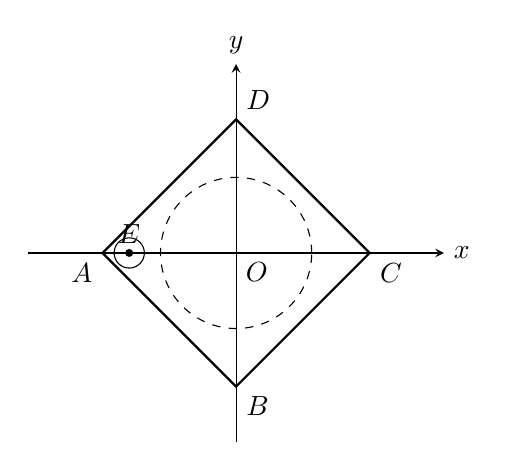
\begin{tikzpicture}[scale=1.2, >=stealth]
  \draw[->] (-2.2, 0) -- (2.2, 0) node[right] {$x$};
  \draw[->] (0, -2.0) -- (0, 2.0) node[above] {$y$};
  \node[below right] at (0,0) {$O$};
  
  % Square ABCD
  \draw[thick] (1.414, 0) node[below right] {$C$} 
    -- (0, 1.414) node[above right] {$D$} 
    -- (-1.414, 0) node[below left] {$A$} 
    -- (0, -1.414) node[below right] {$B$} -- cycle;
    
  % Circle O (r = 0.8)
  \draw[dashed] (0,0) circle (0.8);
  
  % Circle E centered at (-1.414*0.8, 0) = (-1.131, 0) with radius 0.8*0.2 = 0.16
  \draw (-1.131, 0) circle (0.16);
  \fill (-1.131, 0) circle (1.2pt) node[above] {$E$};
  
\end{tikzpicture}
\end{center}

\noindent
(1) 2円が交わる条件は、(2)から、
\[
r - r(1-r) < \sqrt{2}r < r + r(1-r)
\]
\[
\iff 0 < r < 2 - \sqrt{2} \quad (\because (1))
\]

\noindent
(2) $K$ が第2象限にあるとして良い。すると、\\
$K(X, Y)$ として、
\[
\begin{cases}
X = \frac{\sqrt{2}}{4}r (r^2 - 2r - 2) \\
Y = \sqrt{r^2 - X^2}
\end{cases}
\]
である。したがって
\begin{align*}
\cos \frac{\theta}{2} &= \frac{X + \sqrt{2}r}{r(1-r)} = \frac{\sqrt{2}r \left[ \frac{r^2-2r-2}{4} + 1 \right]}{r(1-r)} = \frac{r^2-2r+2}{4(1-r)} \cdot \sqrt{2} \\
&= \frac{\sqrt{2}}{4} \left\{ (1-r) + \frac{1}{1-r} \right\} \tag{3}
\end{align*}
である。$t = 1-r$ に対し、$f(t) = t + \frac{1}{t}$ とすると、(1)のとき $-1+\sqrt{2} < t < 1$ で $y = f(t)$ のグラフは右図だから (1)のとき $2 < f(t) < 2\sqrt{2}$ である。(3)に代入して
\begin{align}
\frac{\sqrt{2}}{2} < \cos \frac{\theta}{2} < 1 \tag{4}
\end{align}
$0 \le \theta \le \pi$ 及び $\cos \frac{\theta}{2}$ が同区間で単調減少なことから、
\[
0 < \frac{\theta}{2} < \frac{\pi}{4}
\]
\[
\therefore 0 < \theta < \frac{\pi}{2}
\]
である。

\begin{center}
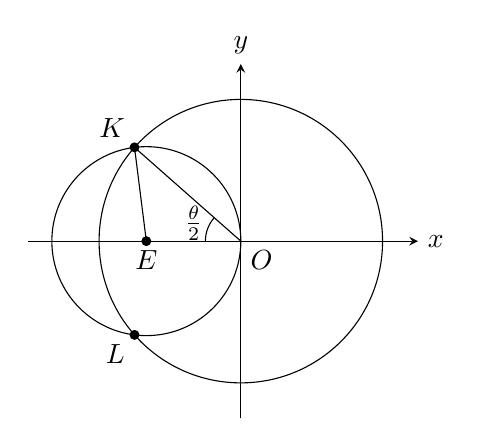
\begin{tikzpicture}[scale=1.5, >=stealth]
  % Circle intersection diagram
  \draw[->] (-1.8, 0) -- (1.5, 0) node[right] {$x$};
  \draw[->] (0, -1.5) -- (0, 1.5) node[above] {$y$};
  \node[below right] at (0,0) {$O$};
  
  \draw (0,0) circle (1.2);
  \draw (-0.8,0) circle (0.8);
  \fill (-0.8,0) circle (1.2pt) node[below] {$E$};
  
  \coordinate (K) at (-0.9, 0.7937);
  \coordinate (L) at (-0.9, -0.7937);
  
  \fill (K) circle (1.2pt) node[above left] {$K$};
  \fill (L) circle (1.2pt) node[below left] {$L$};
  
  \draw (0,0) -- (K);
  \draw (-0.8,0) -- (K);
  
  \draw (0,0) ++(180:0.3) arc (180:138.6:0.3);
  \node at (-0.4, 0.15) {$\frac{\theta}{2}$};
\end{tikzpicture}
\quad
\begin{tikzpicture}[scale=1.5, >=stealth]
  % f(t) = t + 1/t graph
  \draw[->] (-0.3, 0) -- (1.5, 0) node[right] {$t$};
  \draw[->] (0, -0.3) -- (0, 3.2) node[above] {$y$};
  \node[below left] at (0,0) {$0$};
  
  \draw[thick, domain=0.414:1, samples=50] plot (\x, {\x + 1/\x});
  \draw[dashed, domain=0.35:0.414, samples=20] plot (\x, {\x + 1/\x});
  \draw[dashed, domain=1:1.2, samples=20] plot (\x, {\x + 1/\x});
  
  \draw[dashed] (0.414, 0) node[below] {$-1+\sqrt{2}$} -- (0.414, 2.828) -- (0, 2.828) node[left] {$2\sqrt{2}$};
  \draw[dashed] (1, 0) node[below] {$1$} -- (1, 2) -- (0, 2) node[left] {$2$};
  
  \fill (0.414, 2.828) circle (1.2pt);
  \fill (1, 2) circle (1.2pt);
  \node[right] at (1.1, 2.2) {$y = f(t)$};
\end{tikzpicture}
\end{center}

\newpage

\section*{第4問}

% (原稿において第4問の解答は空欄)

\newpage

\section*{第5問}

\noindent
[\textbf{解}] $a > 0 \dots (1)$
\[
\begin{cases}
C_1 : y = x^2 \\
C_2 : x = \frac{1}{6}a^2 y^2 - \frac{7}{6}ay \equiv f(y)
\end{cases}
\]
とおく。$f(y) = \frac{1}{6}a^2 \left( y - \frac{7}{2a^2} \right)^2 - \frac{49}{24a^2}$ だから、グラフの概形は右図

\begin{center}
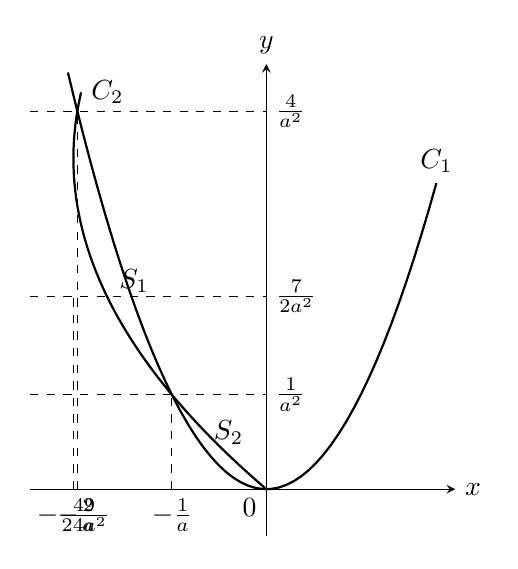
\begin{tikzpicture}[scale=1.2, >=stealth]
  \draw[->] (-2.5, 0) -- (2.0, 0) node[right] {$x$};
  \draw[->] (0, -0.5) -- (0, 4.5) node[above] {$y$};
  \node[below left] at (0,0) {$0$};
  
  \draw[thick, domain=-2.1:1.8, samples=50] plot (\x, {\x*\x}) node[above] {$C_1$};
  
  \draw[thick, domain=0:4.2, samples=50] plot ({1/6*\x*\x - 7/6*\x}, \x) node[right] {$C_2$};
  
  \draw[dashed] (-2.5, 4) -- (0, 4) node[right] {$\frac{4}{a^2}$};
  \draw[dashed] (-2.5, 2.04) -- (0, 2.04) node[right] {$\frac{7}{2a^2}$};
  \draw[dashed] (-2.5, 1) -- (0, 1) node[right] {$\frac{1}{a^2}$};
  \draw[dashed] (-49/24, 0) node[below] {$-\frac{49}{24a^2}$} -- (-49/24, 2.04);
  
  \draw[dashed] (-2, 0) node[below] {$-\frac{2}{a}$} -- (-2, 4);
  \draw[dashed] (-1, 0) node[below] {$-\frac{1}{a}$} -- (-1, 1);
  
  \node at (-1.4, 2.2) {$S_1$};
  \node at (-0.4, 0.6) {$S_2$};
\end{tikzpicture}
\end{center}

\noindent
交点の $x$ 座標について、$y$ を消去して
\begin{align*}
6x &= a^2 x^4 - 7ax^2 \\
x(a^2 x^3 - 7ax - 6) &= 0 \\
x(ax + 1)((ax)^2 - (ax) - 6) &= 0 \\
x(ax + 1)(ax - 3)(ax + 2) &= 0
\end{align*}
\[
\therefore x = 0, \, -\frac{1}{a}, \, -\frac{2}{a}, \, \frac{3}{a}
\]
となる。したがって、右図のように面積 $S_1, S_2$ をおくと、まず
\begin{align}
S_2 = 
\begin{tikzpicture}[scale=0.4, baseline=-0.5ex]
  \draw (0,0) rectangle (1,0.7);
\end{tikzpicture}
-
\begin{tikzpicture}[scale=0.4, baseline=-0.5ex]
  \draw (0,0) -- (1,0) -- (1,0.7);
  \draw (0,0) parabola (1,0.7);
\end{tikzpicture}
-

\begin{tikzpicture}[scale=0.4, baseline=-0.5ex]
  \draw (0,0) -- (0,0.7) -- (1,0.7);
  \draw (0,0) parabola (1,0.7);
\end{tikzpicture}
\tag{2}
\end{align}
となる。対称性に注意して
\begin{align*}
\begin{tikzpicture}[scale=0.4, baseline=-0.5ex]
  \draw (0,0) rectangle (1,0.7);
\end{tikzpicture}
&= \frac{1}{a} \cdot \frac{1}{a^2} = \frac{1}{a^3} \\
\begin{tikzpicture}[scale=0.4, baseline=-0.5ex]
  \draw (0,0) -- (1,0) -- (1,0.7);
  \draw (0,0) parabola (1,0.7);
\end{tikzpicture}
&= \int_0^{\frac{1}{a}} x^2 \, dx = \frac{1}{3}\frac{1}{a^3} \\

\begin{tikzpicture}[scale=0.4, baseline=-0.5ex]
  \draw (0,0) -- (0,0.7) -- (1,0.7);
  \draw (0,0) parabola (1,0.7);
\end{tikzpicture}
&= -\int_0^{\frac{1}{a^2}} f(y) \, dy = -\left[ \frac{a^2}{18}y^3 - \frac{7}{12}ay^2 \right]_0^{\frac{1}{a^2}} = \frac{19}{36}\frac{1}{a^3}
\end{align*}
だから、(2)に代入して
\begin{align}
S_2 = \left( 1 - \frac{1}{3} - \frac{19}{36} \right) / a^3 = \frac{5}{36}\frac{1}{a^3} \tag{3}
\end{align}
一方、$S_1$ について、
\begin{align}
S_1 = 
\begin{tikzpicture}[scale=0.4, baseline=-0.5ex]
  \draw (0,0) rectangle (1.2,0.7);
\end{tikzpicture}
-
\begin{tikzpicture}[scale=0.4, baseline=-0.5ex]
  \draw (0,0) rectangle (1,0.7);
\end{tikzpicture}
\tag{4}
\end{align}
である。
\begin{align*}
\text{[第1領域]} &= -\int_{\frac{1}{a^2}}^{\frac{4}{a^2}} f(y) \, dy = -\left[ \frac{a^2}{18}y^3 - \frac{7}{12}ay^2 \right]_{\frac{1}{a^2}}^{\frac{4}{a^2}} = \frac{21}{4a^3} \\
\text{[第2領域]} &= \left( \frac{8}{a^3} - \frac{1}{a^3} \right) - \int_{\frac{1}{a}}^{\frac{2}{a}} x^2 \, dx = \frac{14}{3a^3}
\end{align*}
を(4)に代入して
\begin{align}
S_1 = \left( \frac{21}{4} - \frac{14}{3} \right) / a^3 = \frac{7}{12}\frac{1}{a^3} \tag{5}
\end{align}
(3),(5)から
\[
S_1 : S_2 = \frac{7}{12} : \frac{5}{36} = 21 : 5 \quad \text{■}
\]

\newpage

\section*{第6問}

\noindent
[\textbf{解}] $g(x) = \alpha x + \beta \quad (\alpha \ne 0, \, \alpha, \beta \in \mathbb{R})$ とおける。条件から、
\begin{align}
\alpha \int_0^a f(x) x \, dx + \beta \int_0^a f(x) \, dx = 0 \tag{1}
\end{align}
が $\alpha \ne 0$ をみたす任意の $(\alpha, \beta)$ で成立するので、(1)が $\alpha, \beta$ についての恒等式となり、
\begin{align}
\int_0^a f(x) \, dx &= 0 \tag{2} \\
\int_0^a f(x) x \, dx &= 0 \tag{3}
\end{align}
である。$f(x) = 0$ が実解を持たない時、$f(x)$ の符号は一定となり、$\alpha \ne 0$ とあわせて(2)はみたされず不適。$f(x) = (x-t)(x-s) \quad (t, s \in \mathbb{R})$ と書ける。$t = s$ の時は $g(x) = x$ とすれば、$f(x)g(x) \ge 0$ (等号は常には成立しない) となり、与式をみたさない。\\
よって $t \ne s$ である。以下、「$t, s$ の少なくとも一方が $x \le 0, a \le x$ にある」と仮定する。\\
この時、これが $t$ だとして良い ($\because$ 対称性)。この時 $g(x) = x - s$ とすると
\[
f(x)g(x) = (x-t)(x-s)^2
\]
の符号は $[0, a]$ で一定であり、与式をみたさず矛盾。よって $0 < t, s < a$ かつ $t \ne s$ となり題意は示された。 \quad \text{■}

\end{document}
